\documentclass[11pt]{article}
\usepackage[margin=2.5cm]{geometry}
\usepackage[T1]{fontenc}
\usepackage{lmodern}
\usepackage{graphicx}
\usepackage{booktabs}
\usepackage{amsmath}
\usepackage{siunitx}
\usepackage[numbers,sort&compress]{natbib}
\usepackage[hidelinks]{hyperref}
\usepackage{setspace}
\onehalfspacing

\title{Which drug--hearing-loss signals in FAERS survive adjustment and independent replication?
A label-referenced, externally replicated disproportionality study}
\author{Oleg Tropynin\\ \small Independent researcher, Karaganda, Kazakhstan\\ \small \texttt{tropininoleg@gmail.com}}
\date{}

\begin{document}
\maketitle

\begin{abstract}
\noindent\textbf{Introduction.} Several recent studies screened the FDA Adverse Event Reporting System (FAERS) for
drug-associated hearing loss using crude disproportionality and reported many unlabelled signals. We asked which signals
survive adjustment for hearing-specific biases and independent replication.

\noindent\textbf{Methods.} We analysed 19.9 million deduplicated FAERS reports (2004--2026) and 1.2 million Canada
Vigilance reports, with a protocol committed before analysis. For hearing loss and tinnitus, crude reporting odds ratios
were compared with Mantel--Haenszel estimates stratified by age, sex and period in a population excluding ear-related
indications, reports naming established ototoxic drugs and lawyer reports. Methods were evaluated against a reference set
from US labels (106 positive, 911 negative ingredients) and by replication in Canada and over time; robust unlabelled
signals underwent case-level review.

\noindent\textbf{Results.} Adjustment changed about a fifth of the 310 crude hearing-loss signals but not agreement with
labels (AUC 0.715 vs 0.717). In Canada, 73\% of labelled and 43\% of unlabelled adjusted signals replicated, as did 21\% of
label-negative drugs, largely through solicited patient-support-programme reports. With both databases adjusted (post hoc),
unlabelled hearing-loss signals replicated at 23\% against a 16\% background. Co-medication bias replicated across databases
(vincristine: crude ROR 1.6 in FAERS and 12.1 in Canada; adjusted 0.45 and 1.15). Of 36 robust unlabelled signals, 26 were
traced to report clusters, ototoxic co-medication, stimulated reporting, indication or an established ototoxic class;
10 remained, led by pregabalin.

\noindent\textbf{Conclusion.} Most unlabelled FAERS hearing-loss signals do not survive adjustment, adjusted replication
and provenance review. Cross-database replication needs adjusted estimates and explicit handling of solicited reports.
\end{abstract}

\section*{Key points}
\begin{itemize}
\item Adjusting FAERS hearing-loss screens for indication, ototoxic co-medication and stimulated reporting changes which
drugs are flagged but does not improve agreement with drug labels.
\item Replication in Canada Vigilance confirms most labelled associations, but solicited patient-support-programme reports
and shared co-medication patterns make about one in five label-negative drugs ``replicate'' too.
\item After adjusted replication and case-level review of report provenance, few unlabelled hearing-loss signals remain;
these, led by pregabalin, are hypotheses for exposure-based studies.
\end{itemize}

\section{Introduction}
Drug-induced hearing loss is usually irreversible, and the classical ototoxic drug classes---aminoglycosides,
platinum agents, loop diuretics, antimalarials, macrolides and salicylates---were identified clinically long before
spontaneous-reporting databases existed \cite{lanvers2017}. For newer drugs, post-marketing spontaneous reports are often
the first source of evidence, and several recent studies have screened the FDA Adverse Event Reporting System (FAERS)
for hearing-loss signals across all drugs \cite{li2024,wu2025,liu2025} and for tinnitus \cite{narasimhaswamy2026}.

Those screens share a design: crude disproportionality across all reports, with novelty defined as absence from the
label. Crude disproportionality in this setting is vulnerable to at least three biases that are specific to hearing
outcomes. First, confounding by indication and protopathic bias: corticosteroids, vasodilators and antivirals are
prescribed \emph{for} sudden hearing loss, tinnitus and vestibular disorders, so they co-occur with the event in reports
for reasons unrelated to toxicity. Second, the ``innocent bystander'' effect: a drug that is routinely co-administered with
a strongly ototoxic one---an antiemetic given with cisplatin, an antibiotic given with an aminoglycoside---inherits part
of the association. Third, stimulated reporting after safety communications or litigation
\cite{pariente2007}. In addition, crude screens rarely test whether their signal list agrees with an independent data
source, and editors have begun to reject FAERS analyses that lack such validation \cite{ramessur2025}.

We therefore asked a narrower question than ``which drugs are ototoxic?'': \emph{which hearing-loss and tinnitus signals
remain after adjustment for these biases, and do the signals that remain replicate in an independent national database
and over time?} We evaluated crude and adjusted detection against a reference set derived from current US labels,
replicated every signal in Canada Vigilance, and compared our results with the signal lists of previous FAERS screens.
The analysis protocol, including all thresholds, was committed to a version-controlled repository (time-stamped
commits) before the first result was computed; the repository is released with this paper.

\section{Methods}
Reporting follows the READUS-PV guideline for disproportionality analyses \cite{readuspv}; the checklist is provided as
Supplementary Table S1.

\subsection{Data sources}
We used all 90 quarterly ASCII extracts of the legacy Adverse Event Reporting System (2004Q1--2012Q3) and FAERS
(2012Q4--2026Q2), the Canada Vigilance Adverse Reaction Online Database extract covering 1965 to 30 June 2026, and the
openFDA bulk export of structured product labels (23 October 2026) \cite{openfda}. All data are public and de-identified;
no ethics approval was required.

\subsection{Pre-processing and deduplication}
In FAERS, we kept the most recent version of each case (by FDA receipt date, preferring FAERS over legacy records, then
case version), removed all case identifiers that FDA lists as deleted, and collapsed content duplicates: reports with
identical sex, age, event date, country, set of suspect ingredients and set of reactions (applied only when event date
and age were present). Drug names were mapped to active ingredients: the \texttt{prod\_ai} field was split into
ingredients, salt and hydrate words were removed when the remaining base was itself an observed ingredient, and
free-text names in records without \texttt{prod\_ai} were mapped to the dominant ingredient seen for that name ($\geq$70\%
of $\geq$5 records). In Canada Vigilance, reports flagged as duplicates of a report present in the extract were removed,
and product ingredients were normalised with the same rules.

\subsection{Outcomes and exposure}
The primary outcome, hearing loss, comprised the MedDRA preferred terms Deafness; Deafness unilateral, bilateral,
neurosensory, transitory, permanent and mixed; Hypoacusis; Neurosensory hypoacusis; Sudden hearing loss; Ototoxicity;
Hearing impaired; Hearing disability; and High frequency hearing loss. Conductive and congenital deafness were excluded.
The secondary outcome was Tinnitus. An ingredient was considered exposed when reported as a suspect drug (FAERS primary
suspect, secondary suspect or interacting; Canada suspect or interacting).

\subsection{Disproportionality}
For each ingredient we computed the reporting odds ratio (ROR) with a Woolf 95\% confidence interval \cite{rothman2004}
and the information component (IC) with its lower credibility bound IC$_{025}$ \cite{noren2006}. A \emph{crude signal}
required at least three cases, a lower ROR bound above 1 and IC$_{025}>0$.

The \emph{adjusted} analysis was run in a restricted population and stratified. We excluded (i) reports in which any
drug had an ear or hearing indication (deafness, hearing, tinnitus, ototoxicity, M\'eni\`ere's disease, otitis, vertigo,
vestibular, labyrinthine and cochlear terms), (ii) reports that mentioned, in any role, a drug from an a-priori list of
29 established ototoxic drugs \cite{lanvers2017} other than the drug under study, and (iii) FAERS reports submitted by
lawyers. We then computed the Mantel--Haenszel OR \cite{mantel1959} over 60 strata (five age bands $\times$ sex
[male, female, unknown] $\times$ four reporting periods) with the Robins--Breslow--Greenland variance
\cite{robins1986}. An \emph{adjusted signal} required at least three cases in the restricted population and a lower
95\% bound above 1. The implementation was checked against \texttt{statsmodels} on simulated data (identical estimates to
nine decimal places).

\subsection{Reference set}
From single-ingredient labels we classified each ingredient as label-positive when a hearing-loss term appeared in a
safety section (boxed warning, warnings, precautions, adverse reactions, post-marketing experience, contraindications,
overdosage, or the corresponding over-the-counter sections) of at least half of its prescription labels, and
label-negative when no label mentioned hearing loss or tinnitus at all; other ingredients were left out. Phrases that
contain a hearing word without describing an adverse effect (for example, the disease name ``maternally inherited
diabetes and deafness'' and telephone lines for deaf users) were removed before matching. Discrimination was assessed
by the area under the ROC curve (AUC) among ingredients with at least 1{,}000 suspect reports, comparing crude IC$_{025}$
with the adjusted lower bound; the difference was bootstrapped (2{,}000 resamples). Because labels are partly informed by
spontaneous reports, the reference set is used to compare methods with each other, not to estimate absolute accuracy.

\subsection{Replication}
For external replication, signals were derived in FAERS after removing reports originating in Canada and tested in
Canada Vigilance. An ingredient was testable when the observed or expected number of Canadian cases was at least three,
and replicated when the Canadian lower ROR bound exceeded 1 with at least three cases. The same rule was applied to
label-negative ingredients that were not FAERS signals, giving the rate at which replication occurs without a true
association. For temporal replication, signals derived from reports received up to 2014 were tested in reports received
from 2015 onwards.

\subsection{Robust signals and novelty}
A \emph{robust signal} was an adjusted FAERS signal that replicated in Canada. Robust signals without a hearing-loss term in
any US label were checked against PubMed (drug name with hearing-loss or ototoxicity terms in title or abstract) and
against the signal lists of the previous FAERS screens \cite{li2024,wu2025,liu2025,narasimhaswamy2026}.


\section{Results}

\subsection{Data}
The 90 FAERS extracts contained 24{,}812{,}424 report versions. Keeping the latest version of each case left
20{,}692{,}682 cases; removing 229{,}233 case identifiers deleted by FDA, cases without a reaction or mappable drug, and
508{,}497 content duplicates left \textbf{19{,}886{,}036 reports} (72.9 million drug rows mapped to 8{,}447 suspect
ingredients; 3.0\% of drug rows could not be mapped). These contained 83{,}914 hearing-loss reports and 42{,}917 tinnitus
reports. The adjusted population excluded 19{,}305 reports with an ear or hearing indication, 1{,}843{,}306 reports
mentioning an established ototoxic drug and 486{,}393 lawyer reports, leaving 17{,}580{,}497 reports
(70{,}459 hearing-loss cases). Canada Vigilance contributed 1{,}210{,}957 reports after removing 58{,}623 duplicates,
with 4{,}001 hearing-loss and 3{,}285 tinnitus reports.

Established ototoxic drugs gave strong signals in both databases (Supplementary Table S2): for example amikacin
(FAERS adjusted OR 12.7, 95\% CI 11.6--13.9), gentamicin (11.4, 9.8--13.2), cisplatin (4.3, 4.0--4.6), the PDE5
inhibitors sildenafil (3.9, 3.7--4.2) and tadalafil (4.2, 3.9--4.6), deferoxamine and teprotumumab. Two
expected positives did not: oxaliplatin (crude ROR 0.44) and, after adjustment, carboplatin (crude 1.96, adjusted 0.82),
whose crude association was carried largely by reports that also named another established ototoxic drug---an
example of the sensitivity that the co-medication filter costs.

\subsection{Adjustment changes the signal list but not its agreement with labels}
In FAERS without Canadian reports, the crude rule flagged 310 ingredients for hearing loss and the adjusted rule 322;
66 crude signals were lost on adjustment and 78 appeared (Table~\ref{tab:methods}). Against the label reference set
(106 positive and 911 negative ingredients with $\geq$1{,}000 suspect reports), discrimination was moderate and
practically identical for the crude IC$_{025}$ (AUC 0.715) and the adjusted lower bound (0.717; difference
+0.003, 95\% CI $-$0.023 to +0.028). Adjustment traded sensitivity (0.40 to 0.35) for specificity (0.86 to 0.87).
Tinnitus showed the same pattern (AUC 0.772 vs 0.776).

\subsection{Replication in a second database}
Adjusted hearing-loss signals that were already labelled replicated in Canada Vigilance in 33 of 45 testable cases
(73\%), unlabelled adjusted signals in 36 of 84 (43\%), crude-only signals in 9 of 21 (43\%), and label-negative
ingredients that were not FAERS signals---the false-replication background---in 48 of 226 (21\%)
(Table~\ref{tab:methods}, Figure~\ref{fig:repl}). Restricting Canada to reports sent directly to Health Canada gave
similar rates (adjusted signals 54\%, background 20\%).

The background was not random. The label-negative ingredients that ``replicated'' were dominated by biologics
(etanercept, rituximab, omalizumab, mepolizumab, ocrelizumab, denosumab) whose Canadian hearing-loss reports came
overwhelmingly from solicited \emph{Study} reports---patient-support programmes run by manufacturers---which made up
93\% of such reports for ocrelizumab and mepolizumab, 86\% for omalizumab, but about 1\% for gentamicin and cisplatin.
The mirror image appeared in FAERS: sacubitril/valsartan (2{,}801 hearing-loss reports; 88\% from consumers) and
tafamidis (361; 86\% consumers) were strong FAERS signals, yet Canada Vigilance recorded 0 sacubitril cases against
1.9 expected and 0 tafamidis cases against 3.4 expected.

In a post-hoc analysis that removed solicited reports from Canada Vigilance and extended the indication filter to
diseases that themselves cause hearing loss (which removed enzyme-replacement therapies for Fabry disease and
mucopolysaccharidoses, canakinumab and cytomegalovirus immune globulin), the background fell to 16\%. When the Canadian
estimate was adjusted in the same way as the FAERS one, labelled signals still replicated in 66\%, but unlabelled
hearing-loss signals replicated in only 12 of 52 (23\%)---close to the 16\% background. For tinnitus the separation was
clearer: 32\% of unlabelled signals against a 7\% background.

Adjusting both databases mattered because co-medication bias replicates. Etoposide and vincristine, given in the same
regimens as cisplatin, were crude signals in both databases (Canada ROR 5.1 and 12.1) and disappeared after adjustment
in both (FAERS adjusted OR 0.78 and 0.45; Canada 1.15 and 1.15). Temporal replication within FAERS did not separate
signal classes at all: early crude-only signals recurred after 2014 at least as often (64\%) as early adjusted ones (52\%),
consistent with biases that persist over time.

\subsection{Signals from previous screens}
Of the 23 hearing-loss signals that Li et al.\ classified as unlabelled \cite{li2024}, 15 were crude and adjusted
signals in our data, 5 were testable in Canada and 2 replicated (clofazimine and glycopyrrolate; Table~\ref{tab:prior}).
Their strongest unlabelled signals included sacubitril/valsartan and tafamidis, discussed above. Of the 28 unlabelled
paediatric signals of Liu et al.\ \cite{liu2025}, 11 survived adjustment in our all-age data; the chemotherapy drugs
etoposide, vincristine, doxorubicin and gemcitabine were among those that did not.

\subsection{Case-level review of robust unlabelled signals}
Under the strict post-hoc definition, 17 hearing-loss and 19 tinnitus signals without any US label mention were adjusted
FAERS signals that replicated in Canada. A rule-based review of their FAERS case series (Figure~\ref{fig:cand},
Supplementary Table S3) attributed 7 to report clusters (most cases in reports listing $\geq$15 drugs; for example
candesartan--tinnitus: 63\% of cases from the United Kingdom, 42\% received in 2023, median 43 drugs per report),
5 to treatment regimens containing established ototoxic drugs (clofazimine, linezolid and rifabutin in mycobacterial
disease with amikacin; mesna with cisplatin; polymyxin B, chiefly as ear drops), 6 to stimulated or mass-exposure
reporting (mRNA COVID-19 vaccines, rofecoxib, finasteride), 7 to an indication or comorbidity linked to the event,
and 1 (oral paromomycin--tinnitus) belongs to an established ototoxic class. Ten remained without an evident explanation
(Table~\ref{tab:cand}): for hearing loss pregabalin, amlodipine, travoprost, glycopyrronium, interferon alfa-2b,
ondansetron and, weakly, etanercept and tocilizumab; for tinnitus clonazepam and procaine benzylpenicillin. Several have
a plausible mechanism or prior clinical descriptions (tinnitus on benzodiazepine withdrawal, auditory symptoms in procaine
reactions, interferon-associated hearing loss), and three (amlodipine, travoprost, glycopyrronium) had at most one PubMed
record linking the drug to hearing loss.

\begin{table}[t]
\centering\small
\caption{Crude versus adjusted detection: reference-set discrimination and replication. Replication counts are
replicated/testable ingredients.}
\label{tab:methods}
\begin{tabular}{p{9.2cm}cc}
\toprule
 & Crude & Adjusted \\
\midrule
\multicolumn{3}{l}{\textit{Hearing loss}} \\
Reference set, positive/negative ingredients & \multicolumn{2}{c}{106/927} \\
AUC, lower 95\% bound & 0.718 & 0.723 \\
\quad difference (95\% CI) & \multicolumn{2}{c}{0.005 (-0.023 to 0.030)} \\
Sensitivity / specificity of the signal rule & 0.40 / 0.87 & 0.35 / 0.87 \\
Signals (FAERS without Canadian reports) & 300 & 310 \\
Replicated in Canada$^a$: labelled adjusted signals & \multicolumn{2}{c}{34/50 (68\%)} \\
\quad unlabelled adjusted signals & \multicolumn{2}{c}{31/76 (41\%)} \\
\quad label-negative adjusted signals & \multicolumn{2}{c}{21/54 (39\%)} \\
\quad crude-only signals & \multicolumn{2}{c}{9/21 (43\%)} \\
\quad background (label-negative non-signals) & \multicolumn{2}{c}{43/214 (20\%)} \\
Observed/expected replications$^b$: labelled & \multicolumn{2}{c}{31/31.2 = 1.00} \\
\quad unlabelled & \multicolumn{2}{c}{25/59.5 = 0.42} \\
\quad label-negative & \multicolumn{2}{c}{18/39.0 = 0.46} \\
\midrule
\multicolumn{3}{l}{\textit{Tinnitus}} \\
Reference set, positive/negative ingredients & \multicolumn{2}{c}{186/927} \\
AUC, lower 95\% bound & 0.775 & 0.777 \\
\quad difference (95\% CI) & \multicolumn{2}{c}{0.002 (-0.015 to 0.019)} \\
Sensitivity / specificity of the signal rule & 0.51 / 0.85 & 0.50 / 0.87 \\
Signals (FAERS without Canadian reports) & 399 & 349 \\
Replicated in Canada$^a$: labelled adjusted signals & \multicolumn{2}{c}{65/89 (73\%)} \\
\quad unlabelled adjusted signals & \multicolumn{2}{c}{24/56 (43\%)} \\
\quad label-negative adjusted signals & \multicolumn{2}{c}{17/43 (40\%)} \\
\quad crude-only signals & \multicolumn{2}{c}{13/30 (43\%)} \\
\quad background (label-negative non-signals) & \multicolumn{2}{c}{31/193 (16\%)} \\
Observed/expected replications$^b$: labelled & \multicolumn{2}{c}{60/64.4 = 0.93} \\
\quad unlabelled & \multicolumn{2}{c}{22/49.4 = 0.45} \\
\quad label-negative & \multicolumn{2}{c}{16/35.5 = 0.45} \\
\bottomrule
\end{tabular}

\smallskip
\raggedright\footnotesize $^a$ Post hoc: FAERS with the extended indication filter; Canada without solicited reports,
adjusted in the same way.
\end{table}

\begin{table}[t]
\centering\small
\caption{Previously reported FAERS hearing-loss signals re-tested in this study. Columns: drugs reported, crude signal
here, adjusted signal here, adjusted and testable in Canada, adjusted and replicated in Canada.}
\label{tab:prior}
\resizebox{\textwidth}{!}{%
\begin{tabular}{llccccc}
\toprule
Study & Authors' label status & Reported & Crude & Adjusted & Testable & Replicated \\
\midrule
Li et al. 2024 (all ages) & labelled & 18 & 18 & 15 & 10 & 10 \\
Li et al. 2024 (all ages) & unlabelled & 23 & 15 & 15 & 5 & 2 \\
Liu et al. 2025 (children) & labelled & 29 & 17 & 17 & 15 & 13 \\
Liu et al. 2025 (children) & unlabelled & 28 & 18 & 11 & 9 & 7 \\

\bottomrule
\end{tabular}}
\end{table}

\begin{table}[t]
\centering\small
\caption{Robust unlabelled signals without an evident artefactual explanation after case-level review. FAERS: adjusted
Mantel--Haenszel OR (extended indication filter, Canadian reports excluded); FAERS cases: all reports naming the drug
as suspect with the event; Canada: ROR without solicited reports; Consumer: share of FAERS cases reported by consumers;
PubMed: records linking drug and event in title/abstract.
These are hypotheses for further study, not evidence of causation.}
\label{tab:cand}
\resizebox{\textwidth}{!}{%
\begin{tabular}{llrcrccr}
\toprule
Drug & Event & FAERS cases & FAERS adj.\ OR (95\% CI) & CA cases & Canada ROR (95\% CI) & Consumer & PubMed \\
\midrule
Etanercept & Hearing loss & 2577 & 1.14 (1.09--1.19) & 111 & 2.25 (1.86--2.72) & 45\% & 35 \\
Pregabalin & Hearing loss & 1795 & 3.21 (3.05--3.38) & 23 & 2.03 (1.35--3.07) & 61\% & 7 \\
Amlodipine & Hearing loss & 841 & 2.33 (2.16--2.52) & 20 & 2.20 (1.41--3.42) & 69\% & 1 \\
Tocilizumab & Hearing loss & 615 & 1.26 (1.13--1.41) & 45 & 1.97 (1.47--2.65) & 41\% & 29 \\
Ondansetron & Hearing loss & 157 & 1.91 (1.57--2.31) & 13 & 4.70 (2.71--8.14) & 40\% & 5 \\
Travoprost & Hearing loss & 143 & 3.61 (3.04--4.28) & 3 & 4.10 (1.31--12.83) & 76\% & 1 \\
Glycopyrronium & Hearing loss & 120 & 2.74 (2.27--3.30) & 5 & 2.92 (1.21--7.05) & 36\% & 1 \\
Interferon Alfa-2B & Hearing loss & 27 & 1.87 (1.26--2.77) & 5 & 2.79 (1.15--6.73) & 22\% & 1 \\
Clonazepam & Tinnitus & 393 & 3.48 (3.11--3.90) & 18 & 3.43 (2.15--5.47) & 69\% & 27 \\
Penicillin G Procaine & Tinnitus & 5 & 7.93 (3.27--19.22) & 5 & 7.72 (3.17--18.79) & 40\% & 3 \\

\bottomrule
\end{tabular}}
\end{table}

\begin{figure}[t]
\centering
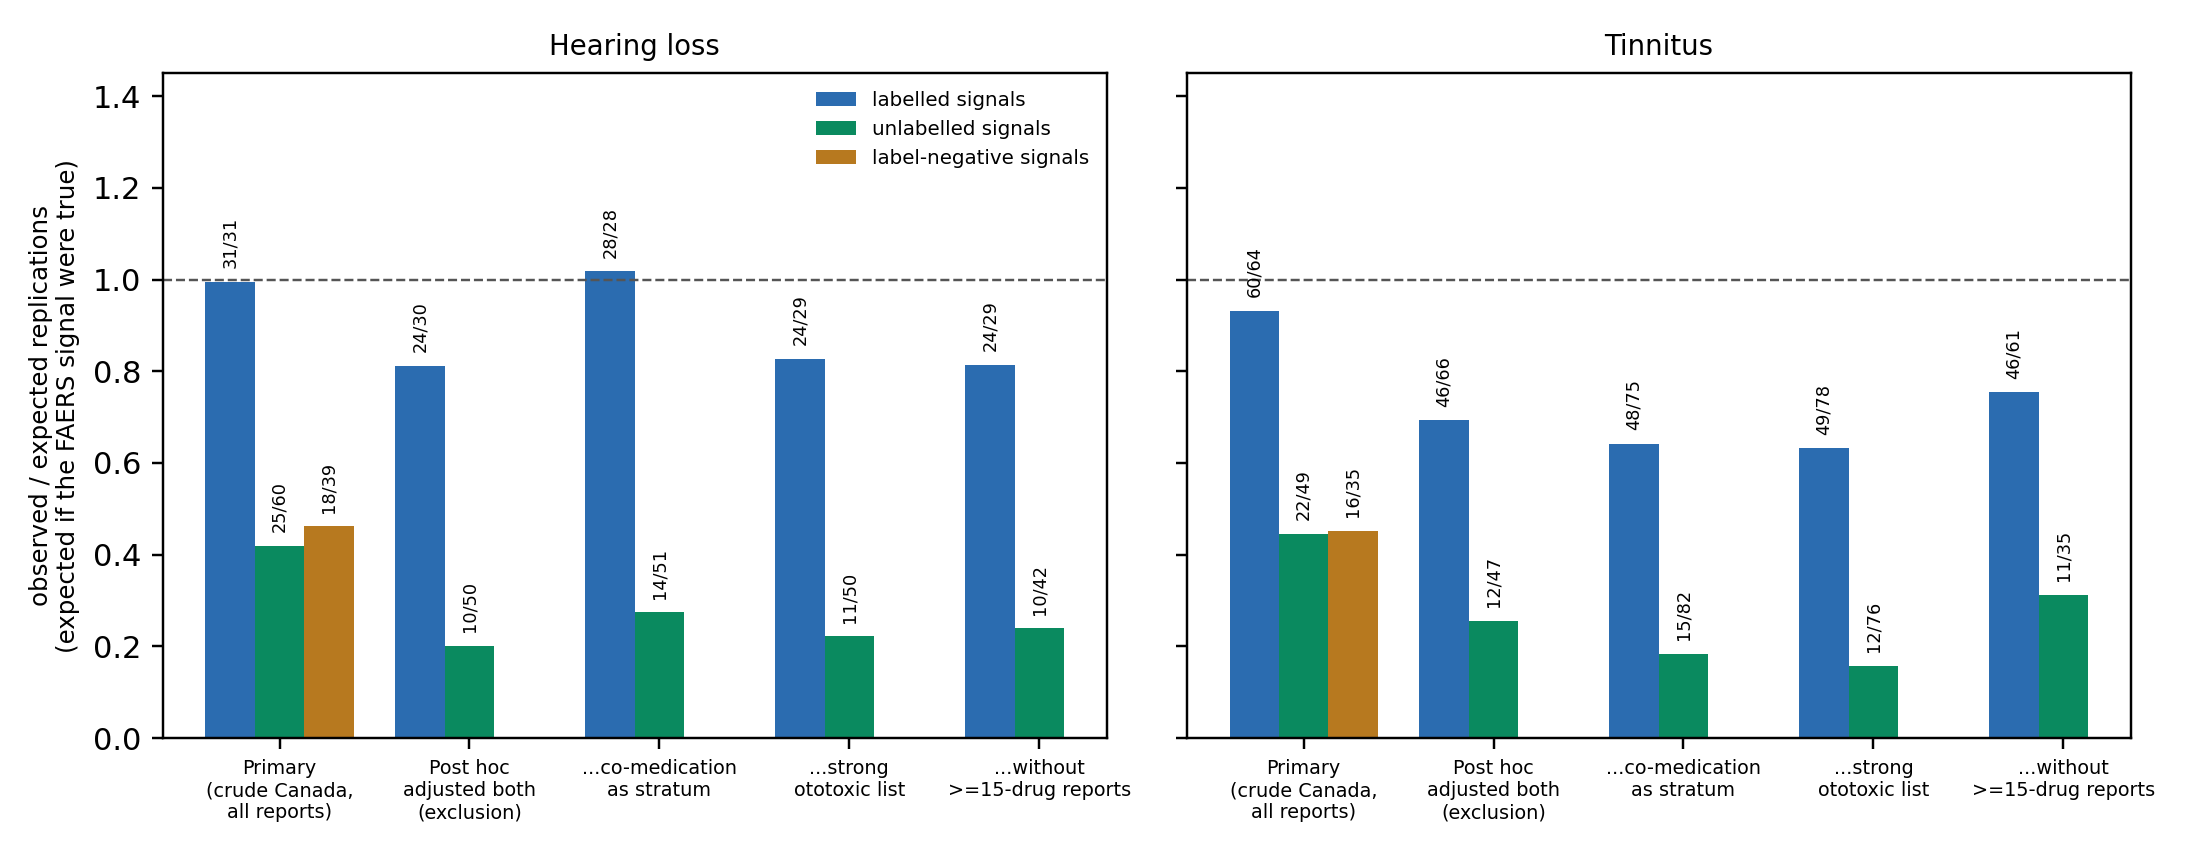
\includegraphics[width=\textwidth]{../figures/replication.png}
\caption{Share of signals replicated, by signal class: in Canada Vigilance (all reports; post hoc without solicited
reports) and in later FAERS reports. Grey bars are label-negative ingredients that were not FAERS signals: the rate at
which ``replication'' happens without a known association.}
\label{fig:repl}
\end{figure}

\begin{figure}[t]
\centering
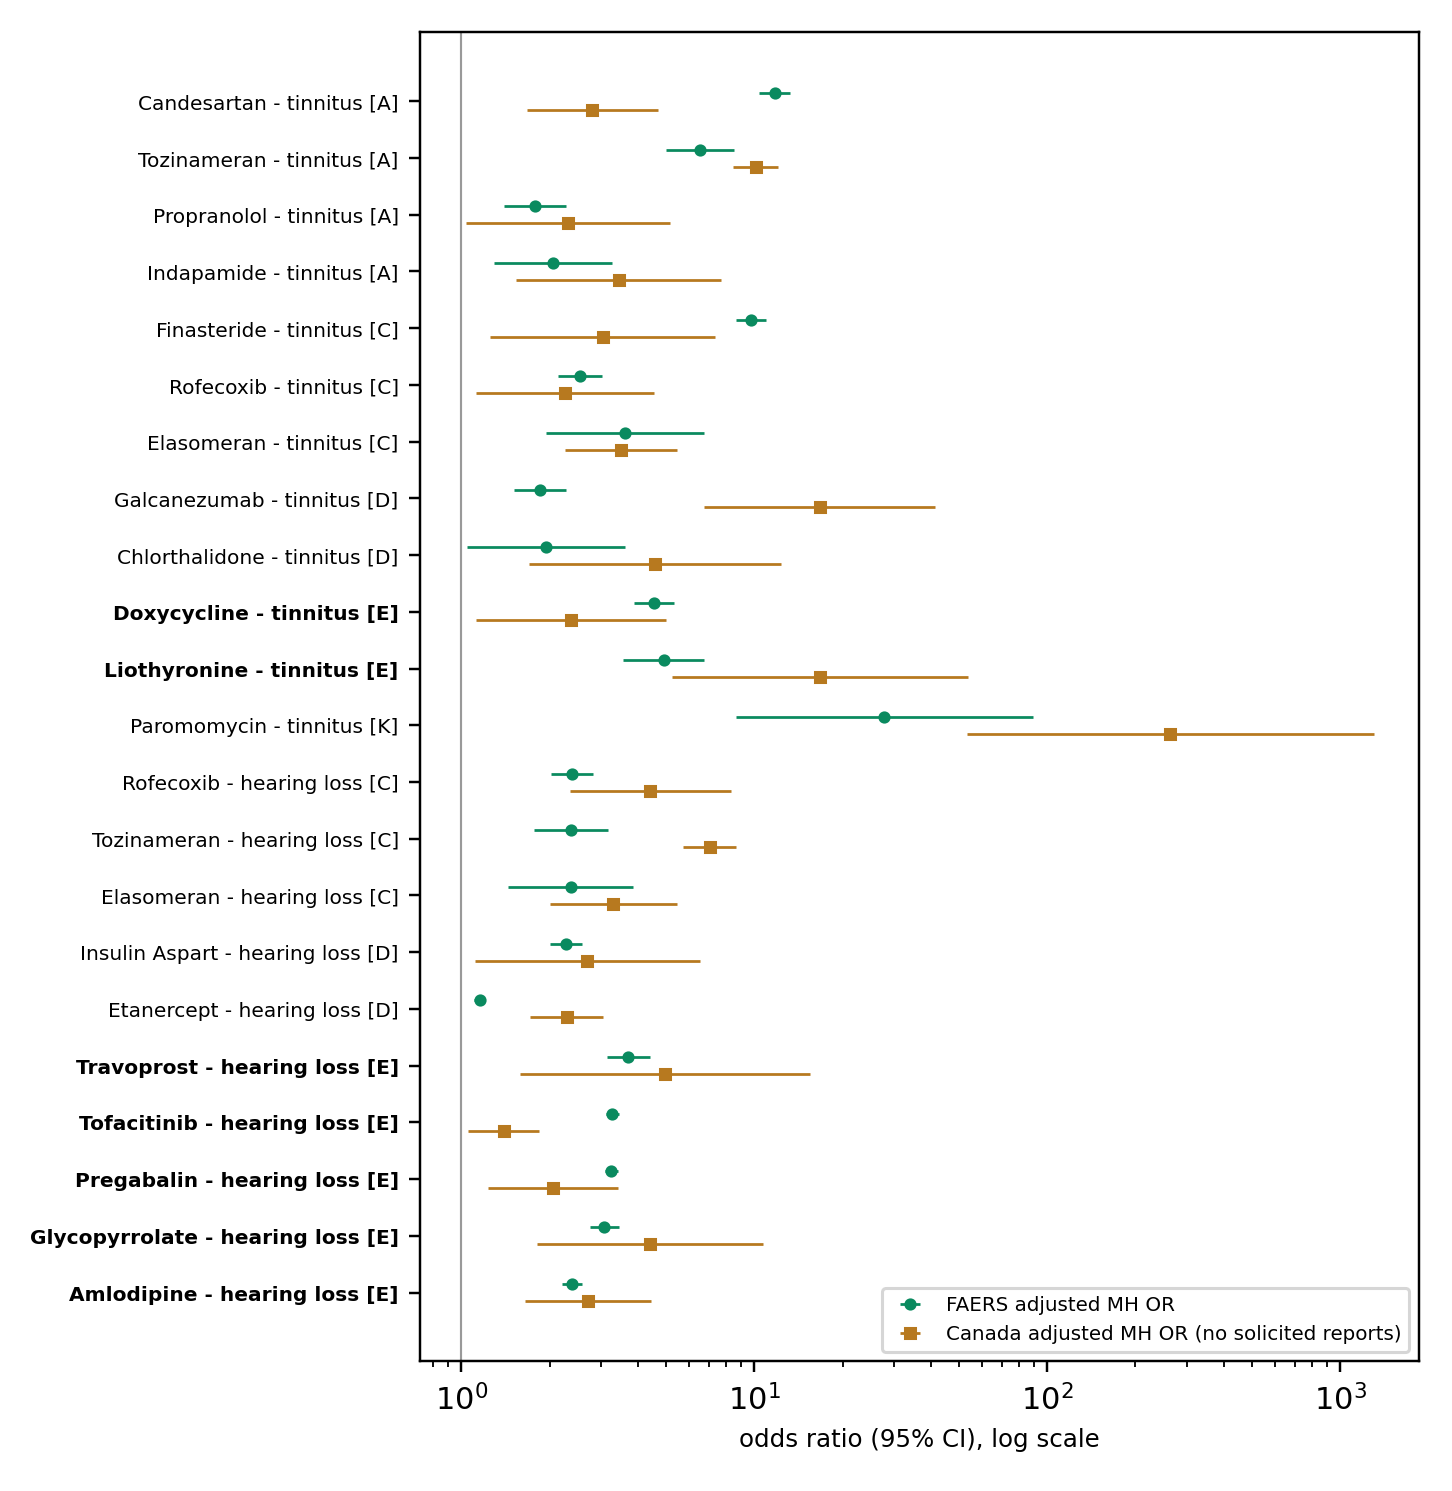
\includegraphics[width=0.85\textwidth]{../figures/candidates.png}
\caption{The 36 robust signals without a US label mention, by case-review category: A report cluster, B co-reported
established ototoxic drug, C stimulated reporting, D indication or comorbidity, K established ototoxic class,
E no evident artefact (bold).}
\label{fig:cand}
\end{figure}



\section{Discussion}
Three findings matter for anyone screening spontaneous reports for ototoxicity. First, adjusting for indication,
ototoxic co-medication, lawyer reports and demographics changed about a fifth of the hearing-loss signal list but did
not improve agreement with labels; crude and adjusted rules were equally (and only moderately) able to separate labelled
from label-silent drugs. Second, replication in an independent national database was informative for labelled
associations---two thirds replicated---but not a clean validator: up to one in five label-negative drugs also
``replicated'', mostly through solicited patient-support-programme reports, and co-medication bias replicated as well
when crude estimates were compared. Third, when both databases were adjusted and solicited reports set aside, unlabelled
hearing-loss signals replicated barely above background, and a case-level review traced most robust unlabelled signals to
identifiable artefacts. The list of credible new hearing-loss signals that an all-drug FAERS screen can support is
therefore short.

These results qualify the previous all-drug screens \cite{li2024,wu2025,liu2025} rather than contradict them. Their
labelled signals largely held; their unlabelled signals mostly did not survive, and some of the strongest ones are
explained by how reports were collected rather than by pharmacology. Sacubitril/valsartan and tafamidis are the clearest
examples: thousands of consumer reports in FAERS, consistent with manufacturer support programmes in the United States,
and none in Canada. The same mechanism produced spurious Canadian ``replications'' for biologics. Report provenance is a
confounder that disproportionality statistics cannot see, and it differs between databases, so it can manufacture both
signals and their replication.

Methodologically, two inexpensive steps removed most of the artefacts we found: comparing \emph{adjusted} estimates in both
databases, and inspecting the case series for concentration---share of solicited or consumer reports, a single country or
year, and very drug-dense reports. The latter flagged report clusters that ordinary deduplication cannot catch because
successive versions differ slightly. We suggest that FAERS screens for hearing outcomes report these provenance indicators
for every signal, in line with the case-by-case review item of READUS-PV \cite{readuspv,readuspv_ee}.

The ten remaining candidates are hypotheses. Some are pharmacologically or clinically familiar (tinnitus during
benzodiazepine withdrawal; auditory symptoms in procaine reactions; interferon-associated hearing loss). Others are less familiar: pregabalin, an $\alpha_2\delta$ ligand with 1{,}795 FAERS
hearing-loss reports that replicated in Canada; the long-acting muscarinic antagonist glycopyrronium; topical travoprost;
and amlodipine, whose labels mention tinnitus but not hearing loss. Each is confounded by age and comorbidity that our
strata capture only coarsely, and none should change practice without pharmacoepidemiological study with exposure data.

\paragraph{Limitations.} Spontaneous reports lack exposure denominators, and disproportionality measures reporting, not risk.
The label reference set is imperfect: labels are partly informed by spontaneous reports, often list rare events without
causal assessment, and route-specific labels (for example topical gentamicin) blur ingredient-level status; we used it
only to compare methods with each other. The indication filter depends on reported indications, which are often missing.
The co-medication filter removes reports with an established ototoxic drug only when it is reported; unreported
co-treatment (for example aminoglycosides in mycobacterial disease) remains. The Canada Vigilance documentation does not
state that the extract is limited to domestic reports; sensitivity analyses restricted to reports submitted directly to
Health Canada gave similar results. Mineral salts were merged at the ingredient level. Part of the analysis---the
solicited-report exclusion, the extended indication filter, adjusted-to-adjusted replication and the case-level review---was
added after the primary results were seen; it is reported as post hoc, and the pre-specified results are given unchanged.

\paragraph{Conclusions.} In FAERS, most drug--hearing-loss signals that are not already on the label do not survive adjustment,
adjusted replication in Canada Vigilance and a review of report provenance. Replication in a second spontaneous-reporting
database is useful only when both estimates are adjusted and solicited reports are handled explicitly. A short list of
candidates---led by pregabalin for hearing loss---merits study with exposure-based designs.


\section*{Declarations}
\textbf{Funding:} none. \textbf{Conflicts of interest:} [TO CONFIRM BY AUTHOR] The author is employed as a software engineer by a company that develops practice-management software for hearing clinics; the company had no role in this work. 
\textbf{Ethics:} not applicable (public, de-identified data).
\textbf{Data and code availability:} all code, the pre-registered protocol and result tables are available at
[REPOSITORY URL --- to be made public before submission].
\textbf{Author contributions:} OT conceived the study, ran the analysis and wrote the manuscript.
\textbf{Use of AI tools:} [TO CONFIRM BY AUTHOR] Data processing code, analyses and a first draft of the manuscript were produced with an AI assistant (Claude, Anthropic) under the author's direction; the author reviewed the code, results and text and takes full responsibility for them.

\bibliographystyle{unsrtnat}
\bibliography{refs}
\end{document}
